La construction d'une plateforme extensive et modulaire pour
démocratiser l'accès à un outil de gestion et de traitement de la donnée
visuelle implique une réflexion approfondie sur les architectures
matérielles et logicielles. Pour toucher des publics diversifiés de la communauté de la recherche, il est
essentiel de penser des infrastructures matérielles diverses, plus ou
moins puissantes et abordables, intégrant ou non des composants comme
les \gpu (qui permettent d'accélérer les calculs intensifs nécessaires à
l'\ia). En effet, la gestion efficace des ressources, la scalabilité,
et la performance sont des aspects à prendre en compte pour
que ces outils puissent être utilisés de manière fiable. Parallèlement, l'architecture logicielle doit être flexible et
évolutive. 

\hypertarget{hardware-une-api-sur-le-gpu}{%
\subsection{Hardware~: une API sur le GPU}\label{hardware-une-api-sur-le-gpu}}

La séparation physique de l'inférence des modèles tient un rôle
important dans l'ouverture de la plateforme.

Le type d'infrastructure de calcul, notamment le \cpu ou le \gpu,
implique des différences dans le traitement et l'analyse des données,
chacun offrant des capacités distinctes adaptées à des besoins
spécifiques. Un \cpu (Central Processing Unit) est le processeur
principal d'un ordinateur, conçu pour gérer une large gamme de tâches
générales et basiques, et utilisé pour les besoins quotidiens. Un \gpu
(Graphics Processing Unit) est spécialisé dans le
traitement des éléments graphiques. Il est conçu pour effectuer un grand
nombre de calculs simples en parallèle grâce à ses nombreux cœurs, ce
qui le rend extrêmement efficace pour des tâches nécessitant un
traitement massif et simultané de données, en particulier la manipulation de matrices ou le calcul vectoriel. L'utilisation d'un \gpu est
souvent nécessaire pour les tâches d'\ia, notamment en vision
artificielle, car ces tâches impliquent souvent des opérations de calcul
intensives et parallélisables. Un \gpu, avec sa capacité à gérer des
milliers de \textit{threads} en parallèle, permet d'accélérer l'entraînement
et l'inférence des modèles de vision artificielle, rendant le traitement
plus rapide et plus efficace que sur \cpu.

Discover-Demo est une \api développée comme un module de l'application, répondant au besoin de séparer les algorithmes de vision du reste
de l'application. Cette séparation permet une plus grande flexibilité
dans l'utilisation des ressources de calcul. Elle tourne sur le \gpu
Dishas-ia, dédié quasi exclusivement aux besoins de l'équipe d'histoire
des sciences du \syrte.

          \begin{figure}[H]
	\begin{center}
		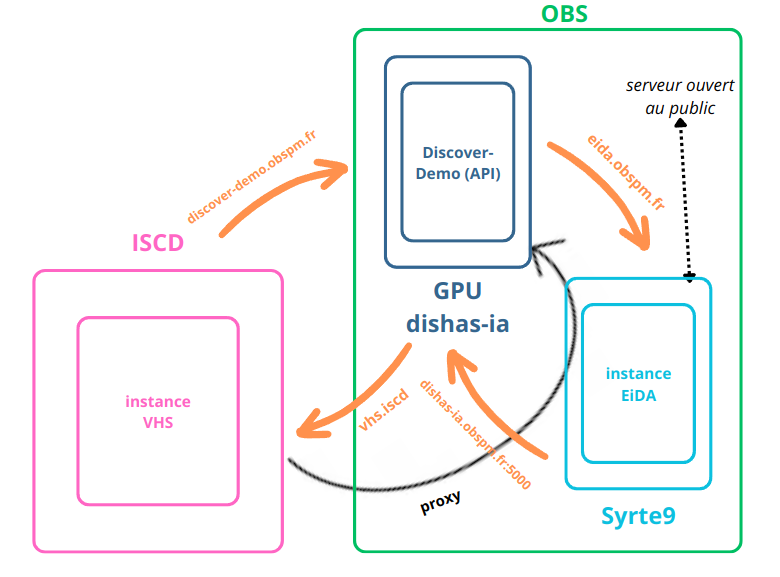
\includegraphics[height=7cm]{figues/com_hard_ware.png}
	\end{center}
	\caption{Organisation et communication des infrastructures.}
	\label{fig:com} \end{figure}

Malgré l'importance accordée à l'\ia,
l'interface web et l'\api associée sont conçues pour une analyse complète
des documents historiques, allant de leur importation et stockage à
leurs traitements (divers) et visualisations. Dans une optique
d'extensivité, elles ne doivent être rattachées à aucun processus d'analyse
prédéterminée. Ainsi, toutes les étapes peuvent être
effectuées manuellement ou à l'aide d'algorithmes automatisés.
L'application de base n'intègre pas de traitement de \cv, mais permet de gérer une base de données et des sources avec
leurs numérisations, utilisant le standard \iiif. Elle permet
l'indexation manuelle de zones d'images dans \sas via l'interface Mirador,
permettant la sélection de zones d'images d'intérêt. Pour cela,
l'extraction automatique de zones d'images est séparée en un nouveau
module, mais les fonctionnalités de base de l'application incluent
toujours les outils nécessaires pour effectuer des annotations manuelles
de régions. Cela comprend toutes les fonctions pour indexer un fichier
texte dans \sas, visualiser les régions annotées, et exporter les
résultats. Il devient alors envisageable d'importer des résultats de traitement
(fichiers d'annotation de régions ou de paires de régions similaires) et
de les indexer manuellement pour permettre leur visualisation et analyse
ultérieure.

Chaque traitement peut donc être
réalisé via l'inférence des modèles de vision sur \gpu (comme c'est le
cas pour \eida grâce à l'\api), par l'import d'un fichier de résultats,
manuellement, ou potentiellement par des méthodes locales sur \cpu
(\yolov, par exemple, est assez léger pour tourner en local). La
plateforme permet ainsi une adaptation à des environnements matériels
divers, laissant la possibilité de réaliser les traitements soit
automatiquement via l'\ia, soit manuellement.

Séparer les modèles de vision c'est aussi permettre une bascule vers des
modèles spécialisés. Les modèles développés dans le cadre du projet sont
disponibles mais peuvent facilement être réentraînés pour correspondre
spécifiquement aux données de l'utilisateur.rice, prenant en compte les
besoins de sa recherche.

Pour conclure, grâce à cette séparation des composants \textit{hard-ware}, la
plateforme répond efficacement à une diversité de besoins et permet son
intégration dans des projets aux ressources matérielles variées. Même
sans ressource matérielle capable de faire tourner les modèles de
vision, les utilisateur.rices peuvent toujours exploiter la plateforme web.
Cette conception offre un accès aux outils et méthode à des utilisateur.rices
divers, allant des projets sans ingénieur dédié pour le
développement, aux équipes de recherche disposant de leurs propres
ingénieurs, en passant par des doctorants indépendants ayant des
compétences en programmation mais sans accès à un serveur. L'outil est
pensé pour s'adapter à des environnements variés, des configurations
légères fonctionnant en local, jusqu'à des projets disposant de
ressources matérielles importantes comme un \gpu.

\hypertarget{software-des-modules-separes}{%
\subsection{Software~: des modules
séparés}\label{software-des-modules-separes}}

Le modèle MVC (Model-View-Controler) est une architecture logicielle qui
segmente une application en trois composantes interconnectées. Le Modèle
est chargé de la gestion des données et de la logique métier de
l'application, assurant la manipulation et l'administration des
informations. La Vue est responsable de la présentation visuelle des
données, les mettant en forme visuellement dans un \textit{template}. Le
'Contrôleur', sert d'intermédiaire entre le 'Modèle' et la 'Vue'~: il reçoit
les entrées de l'utilisateur.rice via la 'Vue', traite ces entrées, puis
interagit avec le 'Modèle' pour actualiser les données et, enfin, met à
jour ces modifications dans la Vue. Cette séparation des préoccupations
permet une organisation plus rigoureuse du code, facilitant ainsi la
maintenance, la réutilisabilité et le développement parallèle de chaque
composante.

Le cycle action → mise à jour → affichage induit par ce patron est bien
adapté aux applications web, il est à ce titre utilisé par nombre
d'entre elles, dont \eida fait partie, et par de nombreux \textit{frameworks},
Django y compris.

Bien que le modèle MVC offre déjà une structure prenant en compte la
séparation des préoccupation, \eida cherche à aller au-delà, proposant
une architecture encore plus flexible. La plateforme est conçue pour
permettre aux développeur.ses d'ajouter ou de supprimer des fonctionnalités
de manière indépendante. Cette approche permet de personnaliser
l'application en fonction des besoins spécifiques de chaque projet, sans
avoir à modifier le cœur du système. Les utilisateur.rices peuvent ainsi
partir de la base de la plateforme et la compléter avec des modules sur
mesure.

Voici une transcription de l'arborescence des fichiers de l'application
:

\begin{verbatim}
app/
├── config/
├── logs/
├── mediafiles/
├── regions/
├── similarity/
├── vectorization/
│   ├── templates/
│   ├── __init__.py
│   ├── const.py
│   ├── tasks.py
│   ├── urls.py
│   ├── utils.py
│   ├── views.py
├── webapp/
├── webpack/
├── __init__.py
├── manage.py
├── requirements-base.txt
├── requirements-dev.txt
├── requirements-prod.txt
cantaloupe/
celery/
docs/
gunicorn/
sas/
scripts/
├── .gitignore
├── .pre-commit-config.yaml
├── README.md
├── run.sh
\end{verbatim}

Il a été créé plusieurs unités fonctionnelles pouvant inclure leurs vues, \textit{templates}, utilitaires, etc. Cette approche
permet aux développeur.ses de découper l'application tout en factorisant le code dédié à
plusieurs tâches, ainsi les modules partagent des \textit{statics}, un fichier
de configuration global et des fonctions utilitaires.

Chaque sous-dossier dans \texttt{app/} représente un module fonctionnel. Le
répertoire \texttt{webapp/} contient le module de base, tandis que \texttt{webpack/} est
dédié aux interfaces\footnote{Voir le \hyperlink{chapitre-8-interfaces}{chapitre suivant}}. Les modules
additionnels, autonomes, peuvent s'interfacer les uns avec les autres,
et être développés puis testés de indépendamment. Pour un exemple
détaillé du contenu des fichiers, une description du module dédié à
la vectorisation développée pendant se trouve en annexe \ref{module_vecto}. 

La variable \texttt{INSTALLED\_APPS} du fichier de configuration global permet de
personnaliser l'application en activant ou désactivant les modules
souhaités.

\emph{Modularité}

Cette architecture s'inscrit dans une stratégie de développement
applicatif ouverte et évolutive. La division en unités fonctionnelles et
indépendantes permet d'ajouter ou de supprimer les fonctionnalités
complémentaires au module de base. Ce cadre de développement modulaire
garantit que l'application reste adaptable aux exigences évolutives des
chercheur.ses et des institutions partenaires, la rendant plus robuste et
tolérante aux usages extérieurs et autorisant alors le réemploi du code
par des projets ayant besoin d'effectuer des traitements divers sur
du matériel documentaire pictural numérisé. \aikon est utilisable par des
projets divers, ce qui réduit le temps de développement et ouvre la voie
à des partenariats, aidant alors à pérenniser les outils.

\emph{Maintenance}

L'organisation modulaire du code facilite également la maintenance et
les mises à jour. Avec une telle structure, il devient plus facile
d'isoler les composants pour le développement et le débogage. Les
développeur.ses peuvent travailler sur un module spécifique sans interférer
avec les autres parties du projet. De plus,
l'implémentation d'un module indépendant provoquera moins de conflit
lors du déploiement.